From the given information, 
\begin{align}
    \norm{\vec{P}-\vec{Q}} &= 3
    \\
    \norm{\vec{R}-\vec{S}} &= 3
    \\
    \norm{\vec{P}-\vec{S}} &= 7.5
    \\
    \norm{\vec{P}-\vec{R}} &= 8
    \\
    \norm{\vec{S}-\vec{Q}} &= 4
    \end{align}
    Let  quadrilateral $PQRS$ be made up of two triangles $\triangle PSQ$ and $\triangle PSR$ on base $PS$.
\begin{enumerate}
        
    \item In $\triangle PSR$,
    \begin{align}
    \norm{\vec{P}-\vec{S}} + \norm{\vec{R}-\vec{S}} &= 7.5 + 3  =10.5 \nonumber \\ &> \norm{\vec{P}-\vec{R}} 
    \\
    \norm{\vec{P}-\vec{R}} + \norm{\vec{R}-\vec{S}} &= 8 + 3 =11 > \norm{\vec{P}-\vec{S}}
    \\
    \norm{\vec{P}-\vec{S}} + \norm{\vec{P}-\vec{R}} &= 7.5 + 8 =15.5 \nonumber \\ & > \norm{\vec{R}-\vec{S}}
    \end{align}
%
    $\therefore$ using triangle inequality, construction of $\triangle PSR$ is possible.

    \item In $\triangle PSQ$,
    \begin{align}
    \norm{\vec{P}-\vec{S}} + \norm{\vec{S}-\vec{Q}} &= 7.5 + 4 =11.5 \nonumber \\ &> \norm{\vec{P}-\vec{Q}} 
    \\
    \norm{\vec{P}-\vec{S}} + \norm{\vec{P}-\vec{Q}} &= 7.5 + 3 =10.5 \nonumber \\ &> \norm{\vec{S}-\vec{Q}}
    \\
    \norm{\vec{P}-\vec{Q}} + \norm{\vec{S}-\vec{Q}} &= 3 + 4 =7 < \norm{\vec{P}-\vec{S}}
    \end{align}
which violates triangle inequality.   $\therefore$ construction of $\triangle PSQ$ is not possible.
    
  
\end{enumerate}

Fig. \ref{constr/32/fig:const_quadrilateral} highlights this.
%
\begin{figure}[!ht]
\centering
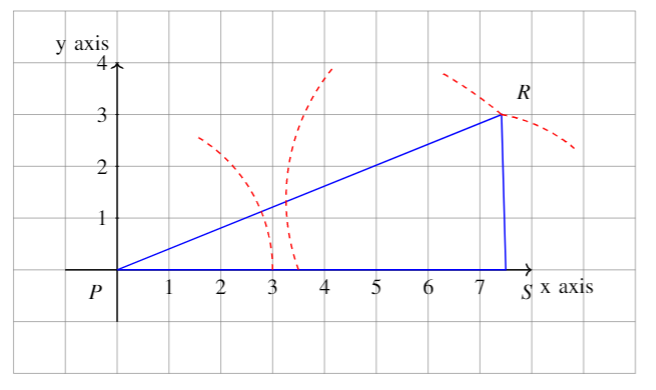
\includegraphics[width=\columnwidth]{solutions/32/Figure2.png}
\caption{Construction of quadrilateral $PQRS$}
\label{constr/32/fig:const_quadrilateral}	
\end{figure}


